% Provenance (never printed): the trade and globalisation strand of ../economics_series.md (grade 6: facts only).
% Brief: sources/book1/BRIEFS.md, g6-07. Chart data: figdata/grade-6/07-a-connected-world (JST R6 exports,
% imports, gdp; WDI NE.TRD.GNFS.ZS, IT.CEL.SETS.P2, IT.NET.USER.ZS; Eurostat prc_hicp_aind; BLS CPI-U;
% cited: the 1927 call, ledger g6:call-london-ny-1927; Brenland accounts and trade).
\chapter{A Connected World}\label{ch:g6:a-connected-world}

Look at the labels of the things around you: a phone assembled in one country
from parts made in ten others, fruit grown on another continent, a shirt sewn
far away. Countries have traded for thousands of years, but never as much as
today. This chapter measures how much countries trade, how the cost of moving
goods and words fell, and how some goods became many times cheaper.

\begin{omfigure}

\includegraphics[width=0.55\linewidth]{images/book1/ai/g6-a-connected-world-call.jpg}

{\small A video call to a grandmother in another country. In 1927, three minutes
of a call between New York and London cost 75 dollars.}
\end{omfigure}

\begin{recall}
A share and the \omterm{def:g6:reading-economic-charts:times-ten-scale}{times-ten scale} were defined in
\cref{ch:g6:reading-economic-charts}, \omterm{def:g6:living-standards:income-per-person}{income per person} in
\cref{ch:g6:living-standards}.
\end{recall}

\section{Selling to and buying from other countries}

\begin{definition}[Export]\label{def:g6:a-connected-world:export}
An \emph{export}\index{export} is a good or a service produced in one country
and sold to buyers in another country.
\end{definition}

\begin{definition}[Import]\label{def:g6:a-connected-world:import}
An \emph{import}\index{import} is a good or a service bought by buyers in one
country from producers in another country.
\end{definition}

The same sale is an \omterm{def:g6:a-connected-world:export}{export} for one country and an \omterm{def:g6:a-connected-world:import}{import} for the other. Services
count too: a tourist from abroad who pays for a hotel room buys an \omterm{def:g6:a-connected-world:export}{export} of the
country she visits.

\begin{definition}[Trade share]\label{def:g6:a-connected-world:trade-share}
A country's \emph{trade share}\index{trade share} is the value of its \omterm{def:g6:a-connected-world:export}{exports}
plus its \omterm{def:g6:a-connected-world:import}{imports} in a year, as a share of the value of everything it produces
in that year (its output):
\[
  \text{trade share} = \frac{\text{exports} + \text{imports}}{\text{output}}
  \times 100\,\%.
\]
\end{definition}

\begin{measure}[Trade as a share of output]
Customs offices record the goods that cross the border, with their value;
surveys of firms, banks and travellers add the services. Output is measured as
in \cref{ch:g8:gdp}. Because \omterm{def:g6:a-connected-world:export}{exports} and \omterm{def:g6:a-connected-world:import}{imports} are added together, the \omterm{def:g6:a-connected-world:trade-share}{trade
share} can be larger than $100\,\%$: a port city that \omterm{def:g6:a-connected-world:import}{imports} goods, works on
them a little and \omterm{def:g6:a-connected-world:export}{exports} them again counts the value twice. In 2024, the \omterm{def:g6:a-connected-world:trade-share}{trade
share} of Singapore was $313.3\,\%$.
% figdata: facts (singapore_trade_2024 313.3)
\end{measure}


\section{Two waves of trade}

\begin{omchart}{Exports plus imports as a share of output, 1870--2024: the
median of eighteen rich economies (1870--2020) and the whole world
(1970--2024).}{Jord\`a--Schularick--Taylor Macrohistory Database (release 6),
\omterm{def:g6:a-connected-world:export}{exports}, \omterm{def:g6:a-connected-world:import}{imports} and GDP; World Bank, World Development Indicators,
NE.TRD.GNFS.ZS}
\begin{tikzpicture}
\begin{axis}[omtime, xmin=1870, xmax=2024, ymin=0, ymax=70,
  xtick={1870,1890,1910,1930,1950,1970,1990,2010}, xlabel={Year},
  ylabel={Percent of output}, legend pos=north west]
\addplot[omThm, thick] table[x=year, y=jst_median]
  {figdata/grade-6/07-a-connected-world/out/trade_share.csv};
\addplot[omExo, thick, densely dashed] table[x=year, y=world]
  {figdata/grade-6/07-a-connected-world/out/trade_share.csv};
\legend{Eighteen rich economies (median), World}
\end{axis}
\end{tikzpicture}
\end{omchart}

The solid line is the middle value of eighteen rich economies of Europe, North
America, Japan and Australia: half of them trade more, half less. The dashed
line covers the whole world, but only from 1970. The chart shows two waves.

% figdata: facts (jst_1870 32.6, jst_1913 41.1, jst_1932 24.9, jst_1945 12.0, jst_1950 35.2,
% jst_2008 59.7, jst_2009 48.3; world_1970 25.8, world_2008 60.3, world_2009 51.9, world_2024 56.7)
In the first wave, trade grew faster than output: the median share rose from
$32.6\,\%$ in 1870 to $41.1\,\%$ in 1913, as railways and steamships carried
grain, cotton and coal across the oceans. Then came the First World War, the
crisis of the 1930s, when countries raised taxes on \omterm{def:g6:a-connected-world:import}{imports}, and the Second World
War: the share fell to $24.9\,\%$ in 1932 and to $12.0\,\%$ in 1945. The second wave
began after 1945. The median share was back at $35.2\,\%$ in 1950 and reached
$59.7\,\%$ in 2008. The world's share rose from $25.8\,\%$ in 1970 to $60.3\,\%$ in
2008. In 2009, during a world crisis, it fell to $51.9\,\%$; in 2024 it was
$56.7\,\%$.

\section{Moving goods and words}

Two things made the waves possible: the cost of moving goods fell, and so did
the cost of sending words and orders across the world.

For goods, the biggest change of the last seventy years was a steel box. A
shipping container has a standard size, so the same box goes from a truck to a
train to a ship and back without being opened. Before containers, gangs of
dockers carried each sack and crate on and off the ship by hand, and a ship
often waited in port for a week or more.

\begin{omfigure}
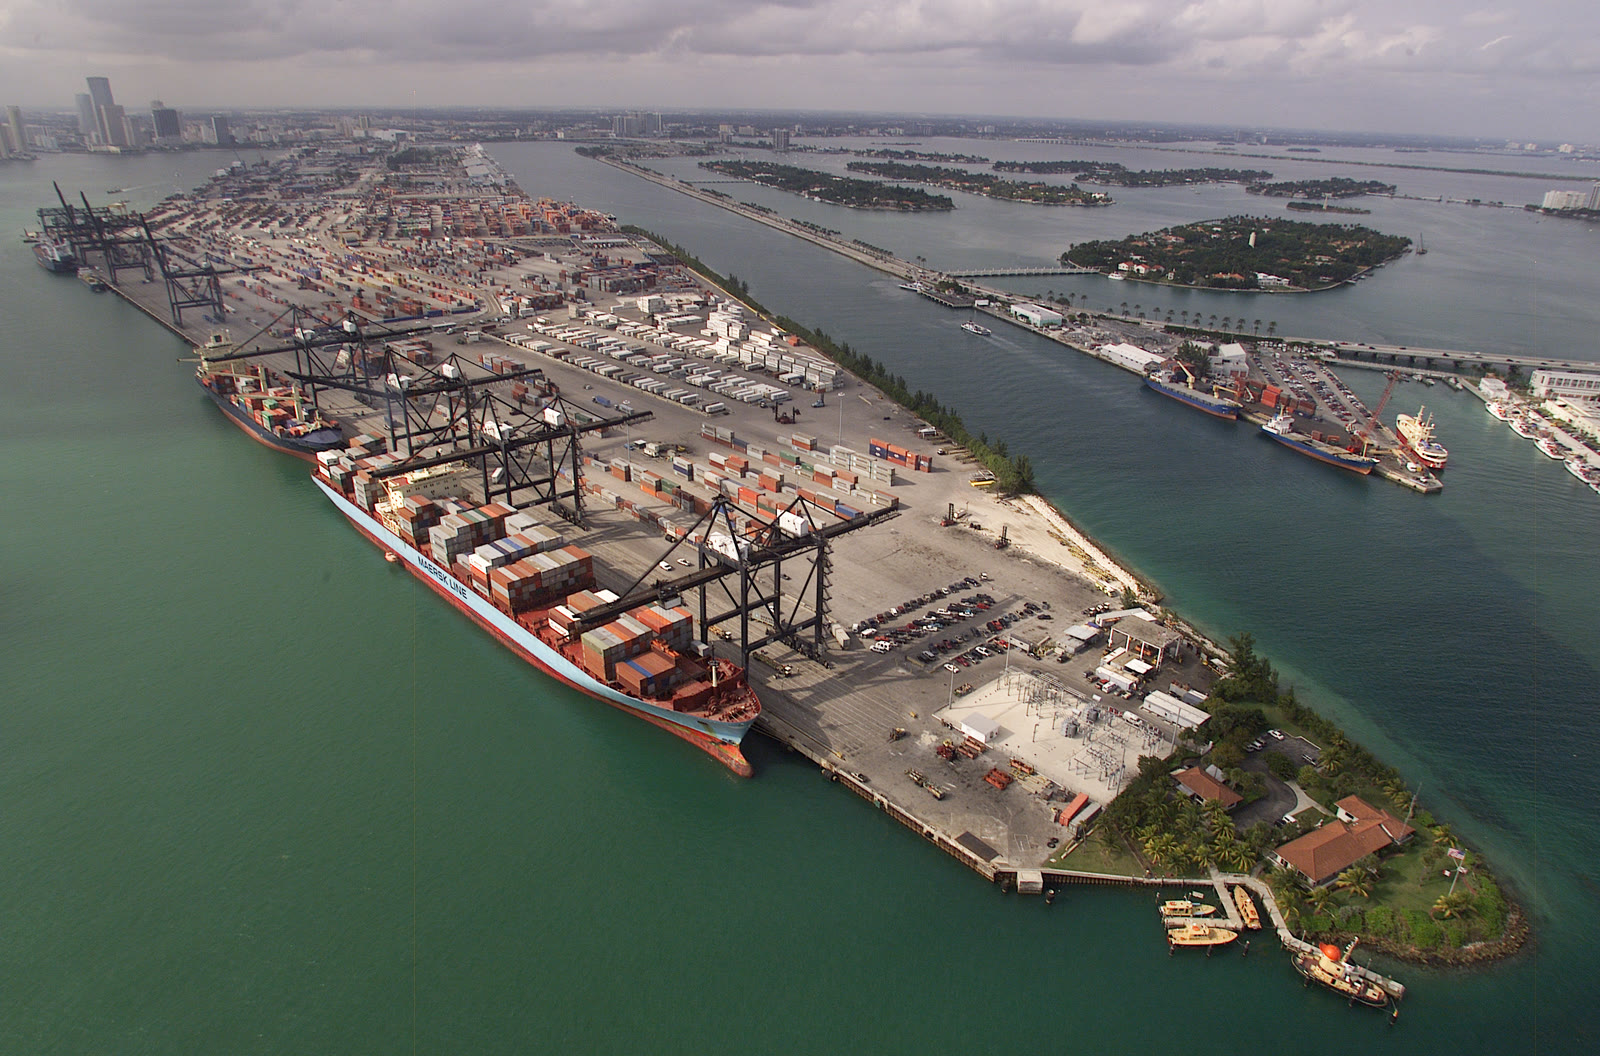
\includegraphics[width=0.55\linewidth]{images/book1/photos/g6-a-connected-world-port-miami.jpg}

{\small A container port. Cranes lift the steel boxes from the ships onto
trucks and trains. Photograph: James R. Tourtellotte, U.S. Customs and Border
Protection, public domain.}
\end{omfigure}

\begin{omfigure}
\begin{tikzpicture}[econ, x=1cm, y=1cm,
  stop/.style={draw, rounded corners=2pt, fill=omMeth!12, align=center,
    font=\scriptsize, minimum width=1.7cm, minimum height=0.9cm}]
  \node[stop] (f) at (0,0) {factory};
  \node[stop] (p1) at (3.0,0) {port};
  \node[stop] (p2) at (7.2,0) {port};
  \node[stop] (w) at (10.2,0) {warehouse\\and shop};
  \draw[-{Stealth}, thick] (f) -- node[above, font=\scriptsize] {truck} (p1);
  \draw[-{Stealth}, thick] (p1) -- node[above, font=\scriptsize] {ship, weeks} (p2);
  \draw[-{Stealth}, thick] (p2) -- node[above, font=\scriptsize] {train} (w);
  % the container, drawn under each leg
  \foreach \x in {1.5, 5.1, 8.7} {
    \draw[fill=omExo!35] (\x-0.35,-0.85) rectangle (\x+0.35,-0.55);
    \foreach \k in {-0.2,0,0.2} \draw (\x+\k,-0.85) -- (\x+\k,-0.55);
  }
  \node[font=\scriptsize, align=center] at (5.1,-1.4)
    {the same box, never opened, on every leg};
\end{tikzpicture}

{\small A container's journey. Only the box is lifted from one vehicle to the
next; the goods inside stay packed from the factory to the warehouse.}
\end{omfigure}

% ledger: g6:call-london-ny-1927 (75 dollars for 3 minutes, 1927)
% figdata: facts (call_1927_dollars 75, cpi_1927 17.4, cpi_2025 321.9, call_1927_in_2025_dollars 1388)
For words, the fall was even larger. When telephone calls between New York and
London opened to the public in 1927, the first three minutes cost 75 dollars. Prices
in the United States have risen a great deal since then: those 75 dollars could buy
as much as about $1\,388$ dollars of 2025. Today, a video call across the world costs
nothing beyond the internet connection.

\begin{omchart}{Mobile phone subscriptions per 100 people (1987--2024) and the
share of people using the internet (2005--2024), the whole world. The world
values for mobile phones are missing for 2000--2004.}{World Bank, World
Development Indicators, IT.CEL.SETS.P2 and IT.NET.USER.ZS, world}
\begin{tikzpicture}
\begin{axis}[omtime, xmin=1987, xmax=2024, ymin=0, ymax=120,
  xtick={1990,1995,2000,2005,2010,2015,2020}, xlabel={Year},
  ylabel={Per 100 people}, legend pos=north west]
\addplot[omThm, thick] table[x=year, y=mobile]
  {figdata/grade-6/07-a-connected-world/out/mobile_early.csv};
\addplot[omExo, thick, densely dashed] table[x=year, y=internet]
  {figdata/grade-6/07-a-connected-world/out/connections.csv};
\addplot[omThm, thick, forget plot] table[x=year, y=mobile]
  {figdata/grade-6/07-a-connected-world/out/connections.csv};
\legend{Mobile phone subscriptions, Internet users}
\end{axis}
\end{tikzpicture}
\end{omchart}

% figdata: facts (mobile_1990 0.2, mobile_2024 110.4, mobile_pass50_year 2007, internet_2005 15.6,
% internet_2024 71.2)
In 1990, there were $0.2$ mobile phone subscriptions for every 100 people in the
world. The number passed 50 in 2007 and reached $110.4$ in 2024: more subscriptions
than people, because some people have two. The share of people using the internet
rose from $15.6\,\%$ in 2005 to $71.2\,\%$ in 2024.

\section{Many times cheaper}

\Cref{ch:g6:living-standards} showed that the light of a lamp became many
thousands of times cheaper in hours of work. Many other goods followed the same
path, if less steeply: once a new product is made in large numbers, its price
keeps falling for decades. Computers are the clearest case of the last thirty
years.

\begin{measure}[A price index]
A \emph{price index} follows how a price changes compared with a starting year,
whose value is set to 100. An index of 50 means that the price is half the
starting price; an index of 4 means that it is 25 times lower. To see whether a
good became cheaper compared with everything else, one divides its price index by
the index of all consumer prices. \Cref{ch:g8:inflation-and-price-indices}
explains how such indices are built.
\end{measure}

\begin{omchart}{Price of computers and other information-processing equipment
compared with all consumer prices, euro area, 1996--2025 (1996 = 100), on a
times-ten scale.}{Eurostat, harmonised index of consumer prices, annual average
indices (prc\_hicp\_aind), euro area: information-processing equipment divided by
all items}
\begin{tikzpicture}
\begin{semilogyaxis}[omtimesten, xmin=1996, xmax=2025, ymin=1, ymax=200,
  xtick={1996,2000,2005,2010,2015,2020,2025}, xlabel={Year},
  ylabel={Index, 1996 = 100}]
\addplot[omThm, thick, mark=*, mark size=1pt] table[x=year, y=index]
  {figdata/grade-6/07-a-connected-world/out/computer_prices.csv};
\end{semilogyaxis}
\end{tikzpicture}
\end{omchart}

% figdata: facts (computers_2025_index 4.01, computers_times_cheaper 24.9)
On this chart, each step down of one gridline means ten times cheaper. Compared
with all the other things that households buy, computers in the euro area cost
in 2025 only $4.01\,\%$ of what they cost in 1996: they became about 25 times
cheaper. The index counts a computer of 2025 as the same good as one of 1996,
corrected for how much more it can do: a faster computer with more memory counts
as more computer.

\section{Prices over time, a first look}

The 75 dollars of the 1927 call show why prices over long periods must be read
with care. A dollar of 1927 bought much more than a dollar of 2025, because most
prices rose in between. To compare, statisticians use a price index of all the
goods that households buy: in the United States, it went from $17.4$ in 1927 to
$321.9$ in 2025, so prices were on average about $18.5$ times higher, and 75
dollars of 1927 match about $1\,388$ dollars of 2025.
% figdata: facts (cpi_1927 17.4, cpi_2025 321.9)
\Cref{ch:g8:inflation-and-price-indices} returns to this. When a book or a chart
in this course compares money across years, it says which year's dollars it uses.

\section{Exercises}

\begin{exercise}[$\star$]\label{exo:g6:a-connected-world:1}
Use the trade chart. About what was the median \omterm{def:g6:a-connected-world:trade-share}{trade share} of the eighteen rich
economies in 1913, and in 1938?
\end{exercise}

\begin{exercise}[$\star$]\label{exo:g6:a-connected-world:2}
Use the trade chart. About what was the world's \omterm{def:g6:a-connected-world:trade-share}{trade share} in 1970, and in 2008?
\end{exercise}

\begin{exercise}[$\star$]\label{exo:g6:a-connected-world:3}
An invented island produces goods and services worth 400 million dalens in a
year. It \omterm{def:g6:a-connected-world:export}{exports} 60 million dalens and \omterm{def:g6:a-connected-world:import}{imports} 100 million dalens. Compute its
\omterm{def:g6:a-connected-world:trade-share}{trade share}.
\end{exercise}

\begin{exercise}[$\star$]\label{exo:g6:a-connected-world:4}
Use the second chart. About what share of the world's people used the internet in
2005, and in 2024?
\end{exercise}

\begin{exercise}[$\star\star$]\label{exo:g6:a-connected-world:5}
% figdata: computer_prices (1996 100, 2006 17.84, 2016 6.42)
The index of computer prices compared with all prices was 100 in 1996, $17.84$ in
2006 and $6.42$ in 2016. (a) How many times cheaper did computers become from 1996
to 2006? Round to one decimal. (b) From 2006 to 2016? (c) Did they become cheaper
faster in the first ten years or in the second?
\end{exercise}

\begin{exercise}[$\star\star$]\label{exo:g6:a-connected-world:6}
An invented port city produces goods and services worth 50 billion dalens. It
\omterm{def:g6:a-connected-world:import}{imports} 70 billion dalens of goods, mostly to work on them and \omterm{def:g6:a-connected-world:export}{export} them again,
and \omterm{def:g6:a-connected-world:export}{exports} 80 billion dalens. (a) Compute its \omterm{def:g6:a-connected-world:trade-share}{trade share}. (b) Explain in one
sentence how a \omterm{def:g6:a-connected-world:trade-share}{trade share} can be larger than $100\,\%$.
\end{exercise}

\begin{exercise}[$\star\star$]\label{exo:g6:a-connected-world:7}
Use the second chart. (a) In which year did mobile subscriptions pass 50 per 100
people? (b) Why can the number of subscriptions per 100 people be larger than 100?
\end{exercise}

\begin{exercise}[$\star\star$]\label{exo:g6:a-connected-world:8}
Someone says: ``Trade between countries always rises.'' (a) Which part of the
trade chart contradicts this? (b) Give the years and the values.
\end{exercise}

\begin{exercise}[$\star\star$]\label{exo:g6:a-connected-world:9}
% figdata: facts (world_2008 60.3, world_2009 51.9)
The world's \omterm{def:g6:a-connected-world:trade-share}{trade share} was $60.3\,\%$ in 2008 and $51.9\,\%$ in 2009. (a) By how
many percentage points did it fall? (A percentage point is the difference between
two percentages: from $30\,\%$ to $25\,\%$ is a fall of 5 percentage points.) (b) The
world's output also fell a little in 2009. What does the fall of the \omterm{def:g6:a-connected-world:trade-share}{trade share}
say about trade compared with output that year?
\end{exercise}

\begin{exercise}[$\star\star\star$]\label{exo:g6:a-connected-world:10}
The price of an invented gadget is 640 dalens. It halves every 5 years. (a) Give its
price after 5, 10, 15 and 20 years. (b) How many times cheaper is it after 20 years?
(c) On a \omterm{def:g6:reading-economic-charts:times-ten-scale}{times-ten scale}, what does the line of this price look like?
\end{exercise}

\begin{exercise}[$\star\star\star$]\label{exo:g6:a-connected-world:11}
% figdata: facts (jst_1945 12.0, jst_1950 35.2, jst_2008 59.7)
The median \omterm{def:g6:a-connected-world:trade-share}{trade share} of the eighteen rich economies was $12.0\,\%$ in 1945,
$35.2\,\%$ in 1950 and $59.7\,\%$ in 2008. (a) By how many percentage points did it
rise from 1950 to 2008? (b) Why is 1945 a misleading starting year for measuring
the second wave?
\end{exercise}

\begin{exercise}[$\star\star\star$]\label{exo:g6:a-connected-world:12}
The trade chart shows that countries trade more and more. (a) Name two questions
about trade that this chart cannot answer. (b) For one of them, say what data
would help.
\end{exercise}

\section{Problem: A Container from Kestria}

\begin{problem}[{Weekend problem --- Brenland's trade, the cost of shipping and
calling, and a gadget that keeps getting cheaper}]
\label{pb:g6:a-connected-world:1}
Brenland and Kestria are the series' invented countries, and every number in
this problem is invented. Part I uses Brenland's national accounts.

\medskip
\noindent\textbf{Part I --- Brenland's trade.} The table gives Brenland's output,
\omterm{def:g6:a-connected-world:export}{exports} and \omterm{def:g6:a-connected-world:import}{imports}, and its \omterm{def:g6:a-connected-world:export}{exports} to and \omterm{def:g6:a-connected-world:import}{imports} from Kestria, in millions of
dalens:

% figdata: brenland_trade (2000: 152000, 48640, 48918, 15078, 13208; 2025: 393264, 129777, 128664, 40231, 34739)
\begin{center}
\begin{tabular}{lrrrrr}
\toprule
Year & Output & \omterm{def:g6:a-connected-world:export}{Exports} & \omterm{def:g6:a-connected-world:import}{Imports} & \omterm{def:g6:a-connected-world:export}{Exports} to Kestria & \omterm{def:g6:a-connected-world:import}{Imports} from Kestria \\
\midrule
2000 & 152\,000 & 48\,640 & 48\,918 & 15\,078 & 13\,208 \\
2025 & 393\,264 & 129\,777 & 128\,664 & 40\,231 & 34\,739 \\
\bottomrule
\end{tabular}
\end{center}
\begin{enumerate}
  \item Compute Brenland's \omterm{def:g6:a-connected-world:trade-share}{trade share} in 2000 and in 2025, to one decimal.
  \item What share of Brenland's \omterm{def:g6:a-connected-world:export}{exports} went to Kestria in 2025? Round to one
        decimal.
  \item In 2025, did Brenland sell more to Kestria than it bought from it? By how
        much?
  \item Output and \omterm{def:g6:a-connected-world:export}{exports} both grew a great deal from 2000 to 2025. Explain why the
        \omterm{def:g6:a-connected-world:trade-share}{trade share} hardly changed.
\end{enumerate}

\medskip
\noindent\textbf{Part II --- Shipping and calling.} A container holds 20 tonnes of
goods. In 1970, sending a container from Kestria to Brenland cost 4\,000 dalens; in
2025, it costs 1\,600 dalens. A three-minute call to Kestria cost 30 dalens in 1970
and costs nothing now (beyond the internet connection).
\begin{enumerate}[resume]
  \item What did shipping one tonne cost in 1970, and in 2025?
  \item By what percent did the cost of shipping a container fall?
  \item A Brenland shop sells a Kestrian bicycle for 300 dalens. A container holds
        200 bicycles. In 2025, what part of the price of one bicycle is the cost of
        shipping it, in dalens and as a share of the price?
  \item The call cost 30 dalens for three minutes. What did ten minutes cost, if
        each minute cost the same?
\end{enumerate}

\medskip
\noindent\textbf{Part III --- A gadget that keeps getting cheaper.} A Kestrian gadget
cost 2\,000 dalens in 2005. Its price was divided by 2 every 4 years.
\begin{enumerate}[resume]
  \item Give its price in 2009, 2013, 2017, 2021 and 2025.
  \item How many times cheaper was it in 2025 than in 2005?
  \item On a \omterm{def:g6:reading-economic-charts:times-ten-scale}{times-ten scale}, would the points of the price lie on a straight line?
        Explain.
  \item Write two sentences explaining why cheaper shipping and cheaper calls help
        Brenland's shops sell Kestrian goods.
\end{enumerate}
\end{problem}
